\section{Method}
\begin{figure*}[t]
\centering
\resizebox{\linewidth}{!}{%
\begin{tikzpicture}[
  font=\scriptsize, >=stealth, node distance=4mm,
  box/.style={draw, rounded corners=2pt, align=center, minimum height=7mm, inner sep=2pt, fill=white},
  data/.style={box, fill=gray!10},
  net/.style={box, fill=blue!8},
  sim/.style={box, fill=orange!12},
  loop/.style={draw, dashed, rounded corners=4pt, inner sep=3pt, blue!50!black}]
% inputs, each tokenised in its canonical frame and encoded with local attention
\node[data, text width=24mm] (A) {snapshot $a$:\\$\{\mathbf{x}_i\}_{i\le N_a}$, tokens + local attention};
\node[data, text width=24mm, below=5mm of A] (B) {snapshot $b{=}a{+}H$:\\$\{\mathbf{y}_j\}_{j\le N_b}$, tokens + local attention};
\node[data, text width=24mm, below=4mm of B] (I) {image at $b$};
% loop: X1 -> U -> X2 -> X1
\node[net, right=15mm of A] (X1) {(i, ii) ancestors attend\\to targets near $\mathbf{c}_i^{(t-1)}$};
\node[net, right=4mm of X1] (U) {(iii) $\mathbf{c}_i^{(t)}{=}\mathbf{c}_i^{(t-1)}{+}\Delta_t$};
\node[net, below=5mm of X1] (X2) {(iv) targets attend\\to nearest centres};
\node[loop, fit=(X1)(U)(X2), label={[blue!50!black, font=\scriptsize]below right:{family registration, $t{=}1..T$}}] (L) {};
\node[net, right=6mm of U] (S) {scores $p_{ji}$\\+ dustbin};
\node[net, right=4mm of S] (P) {Potts mean\\field (Eq.~1)};
\node[box, right=4mm of P] (O) {ancestor\\$\pi(j)$};
% genealogy
\node[net, right=6mm of I] (G) {pair CNN: $P(\tau_{jk}{<}H)$};
% real-data inset: centres moving through the rounds
\node[anchor=north west, inner sep=0] (IN) at ([xshift=4mm, yshift=-3mm]O.north east) {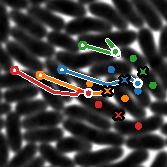
\includegraphics[height=29mm]{fig/centre_inset.pdf}};
\node[anchor=south, font=\scriptsize] at (IN.north) {real data, $H{=}66$ min};
\draw[->] (A) -- node[above, font=\scriptsize] {$\mathbf{c}^{(0)}_i$} node[below, font=\tiny] {radial/Darcy} (X1);
\draw[->] (I) -- (G);
\draw[->] (X1) -- (U);
\draw[->] (U.south) |- (X2.east); \draw[->] (X2.north) -- (X1.south);
\draw[->] (B) -- (X2);
\draw[->] (U) -- (S); \draw[->] (S) -- (P); \draw[->] (G) -| (P); \draw[->] (P) -- (O);
\end{tikzpicture}}
\caption{\textbf{Overview.} For every ancestor \ours keeps one estimate of its descendant-family centre and refines it over $T$ rounds of cross-attention to nearby targets; targets then score candidate ancestors by their offset from the refined centres. A genealogy network predicts from the target image whether neighbouring cells share an ancestor $H$ minutes ago, and a Potts mean-field decoder combines both. The same network is trained on \rodsim colonies, self-labelled time-lapses or annotated lineage. Right: in a dense OIAM window, centres move from initialisation (open) to $\mathbf{c}_i^{(T)}$ (filled) towards the true centroids (crosses) of the descendants (dots).}
\label{fig:method}
\end{figure*}

\label{sec:method}

\subsection{\ours: iterative family registration}
\label{sec:raft}

\paragraph{Tokens.}
\cref{fig:method} gives an overview. Each cell becomes a token built only from quantities available in its own snapshot, plus four scalars shared by the window: $\log_2 H$, $\log(N_b/N_a)$, $\log N_a$ and $\log N_b$.
Positions are expressed in a canonical frame: centred on the snapshot centroid and divided by the median nearest-neighbour spacing $s$; ancestor positions are additionally scaled by $\sqrt{N_b/N_a}$, the isotropic expansion that keeps the population density constant.
Per-cell features add orientation as $(\cos 2\theta,\sin 2\theta)$, log major and minor axes (when shapes are used), and the vector to the nearest image border, through which cells leave.

\paragraph{Encoder.}
Two layers of local attention operate within each snapshot: every token attends to its $k{=}12$ nearest neighbours, with keys and values augmented by an MLP embedding of the relative offset.
A global context token, pooled over the snapshot, is broadcast back.

\paragraph{Iterative family registration.}
Let $\mathbf{c}_i^{(0)}$ be an initial estimate of the centre of ancestor $i$'s descendant family at time $b$ (the scaled position above, or the advection of $\mathbf{x}_i$ through a Darcy growth-pressure field, \cref{sec:darcy}).
For $t=1,\dots,T$ ($T{=}4$):
(i) ancestor $i$ cross-attends to the $24$ targets nearest $\mathbf{c}_i^{(t-1)}$, with relative offsets $\mathbf{y}_j-\mathbf{c}_i^{(t-1)}$ as positional keys;
(ii) ancestors exchange information with their spatial neighbours;
(iii) the centre is updated, $\mathbf{c}_i^{(t)}=\mathbf{c}_i^{(t-1)}+\Delta_t(\mathbf{h}_i)$, with a zero-initialised head;
(iv) targets attend to their nearest centres, so a target's representation knows which families compete for it.
Updating a single point per family, rather than a dense field, matches the structure of the problem: families move rigidly to first order while the population as a whole deforms non-uniformly.

\paragraph{Assignment.}
Each target $j$ is scored against the $k_{\text{out}}{=}24$ ancestors whose final centres are closest, by an MLP over $[\mathbf{h}_j,\mathbf{h}_i,(\mathbf{y}_j-\mathbf{c}_i^{(T)})/4,\|\mathbf{y}_j-\mathbf{c}_i^{(T)}\|/4]$, plus a learned dustbin logit for targets without a visible ancestor~\cite{sarlin2020superglue}.

\paragraph{Training.}
Windows are sampled from every pair of frames with $H$ log-uniform in $[8,240]$ minutes.
The loss combines cross-entropy over candidates and dustbin, a deeply supervised centre loss $\sum_t 0.8^{T-t}\min(\|\mathbf{c}_i^{(t)}-\bar{\mathbf{y}}_{\mathcal{F}(i)}\|,10)$ towards the true family centroid $\bar{\mathbf{y}}_{\mathcal{F}(i)}$ (the mean position of $i$'s descendants), a binary same-family loss on target pairs, and an optional consistency term that asks the assignment overlap $\sum_i p_{ji}p_{ki}$ to agree with family membership.
Models trained on \rodsim or for transfer are augmented with random rotations and reflections of the canonical frame; in-domain OIAM models are trained without them, since the growth chambers fix a preferred axis.

\subsection{\rodsim: randomised colony simulation}
\label{sec:sim}

\rodsim grows colonies of rod-shaped cells from one to four founders until 900--2{,}200 cells.
Each cell is a chain of spheres of radius $0.5\,\mu$m; overlapping cells repel through soft contacts with anisotropic drag and torque, and elongate exponentially at a rate drawn around a doubling time of 40--110 minutes with cell-to-cell variation.
Cells divide by an adder rule into two daughters with a small angular perturbation.
An extended version (\emph{division modes}) additionally randomises the position of the division plane (asymmetric division), a V-shaped opening of the daughters around the septum (V-snapping), a cell width inherited with noise, and per-frame measurement noise on lengths, widths and orientations; each mechanism ranges from absent to strong, so symmetric \emph{E.~coli}-like division remains part of the distribution.
Per colony we randomise birth length, doubling time, growth and adder noise, division angle noise, translational and rotational diffusion, drag anisotropy, pixel size, and a field of view that crops the colony at a random scale and offset, so that cells leave through image borders as they do in microfluidic chambers.
We simulate 256 colonies (about 1.5 CPU-hours) and sample training windows exactly as for real movies.
The simulator was designed from first principles and generic literature values; none of its parameters was fitted to an evaluation dataset, but leaving division modes out of the assignment simulator was decided after zero-shot evaluation (Supp.~K).

\subsection{Self-labelling from unannotated time-lapses}
\label{sec:selflabel}
Lineage is hard to infer across hours but nearly trivial across one frame of a dense time-lapse, and binary fission constrains it further: a cell has one successor, or two daughters lying on either side of its old centre along its axis.
Given an unannotated dense time-lapse with detections only, we link every pair of consecutive frames by an exact linear assignment in which each cell $i$ of frame $t$ offers three slots, \emph{stay} at $\mathbf{x}_i$ and two \emph{daughter} slots at $\mathbf{x}_i\pm\tfrac{L_i}{4}\mathbf{u}_i$ (length $L_i$, axis $\mathbf{u}_i$) that cost an extra $0.55s$, plus a no-parent option at $3.5s$, where $s$ is the nearest-neighbour spacing.
Without masks, the daughter slots sit at $\mathbf{x}_i$.
Where cells move far between frames, \emph{temporal bootstrapping} replaces these one-frame links by the \rodsim model's own one-frame predictions.
Composing the one-frame links gives pseudo-ancestry between any two frames, and we train \ours on it exactly as on annotated lineage.
The dense movie is needed once per organism or condition; experiments then need only snapshots.

\subsection{Single-snapshot genealogy}
\label{sec:genealogy}

For neighbouring cells $(j,k)$ in one snapshot let $\tau_{jk}$ be the time since their lineages split.
Two targets share an ancestor $H$ minutes earlier if and only if $\tau_{jk}<H$, so predicting $\tau$ once serves every horizon.
We predict the cumulative events $\tau<\{8,16,33,66,132,264\}$ for the $8$ nearest neighbours of each cell from a $64{\times}64$ patch aligned with the pair axis and centred on its midpoint (plus a channel marking the two cells) and ten pair-geometry features, with a small CNN and MLP.

\paragraph{Partition-aware decoding.}
Let $p_{ji}$ be \ours's assignment probabilities and $w_{jk}$ the genealogy probability for horizon $H$.
We run Potts mean field
\begin{equation}
q_j \propto p_j \odot \exp\Big(\beta\sum_{k\in\mathcal{N}(j)}(2w_{jk}-1)\,q_k\Big)
\end{equation}
over the 8 nearest neighbours $\mathcal{N}(j)$ of $j$ for ten iterations and assign $\arg\max q_j$.
Likely relatives pull a target towards their ancestor, non-relatives push it away.

\subsection{Darcy growth-pressure prior}
\label{sec:darcy}
A dense growing monolayer behaves like an active porous medium~\cite{volfson2008biomechanical,delarue2016selfdriven}: local growth $g$ creates pressure $-\nabla^2 p=g$ inside the colony with $p{=}0$ on free boundaries, and cells move with $\mathbf{v}=-\nabla p$.
We set $g{=}\ln(N_b/N_a)/H$ when both snapshots show the whole colony and a fixed 68-minute doubling time otherwise, solve on a grid and advect ancestors for $H$ minutes, which gives a physically grounded initial centre $\mathbf{c}_i^{(0)}$.
